% =============================================================================
%  Paper A — the predictive line of Mol-Metal
%
%  "Few-shot metal adaptation (FSMA) recovers cross-metal collapse"
%
%  Target journal: J. Chem. Inf. Model. (ACS)  [fallback: Digital Discovery]
%  Plan + scope: docs/SUBMISSION_PLAN.md, docs/PAPER_SCOPE.md,
%                docs/ALIGNED_COMPARISON.md
%
%  This is a NEW manuscript. It deliberately does NOT reuse paper/ (which holds
%  the old single-paper lambda-calculus + CFM narrative, i.e. Paper B's
%  material). Per AGENTS.md §5.3 / TODO-84 the paper/ tree is untouched.
%
%  Honest framing (AGENTS.md §5.2): every quantitative claim is tagged
%  \textbf{MEASURED} or \textbf{PROJECTED} at the point of use, and every number
%  cites an on-disk source under metrics/by_metric/.
% =============================================================================

\documentclass[11pt]{article}

\usepackage[T1]{fontenc}
\usepackage{amsmath,amssymb}
\usepackage{graphicx}
\graphicspath{{figures/}{./}}
\usepackage{booktabs}
\usepackage[margin=1in]{geometry}
\usepackage[round,numbers]{natbib}
\bibliographystyle{unsrtnat}
\usepackage{hyperref}
\usepackage{xcolor}

\newcommand{\MEASURED}{\textbf{MEASURED}}
\newcommand{\PROJECTED}{\textbf{PROJECTED}}
\newcommand{\fsma}{\textsc{fsma}}

\title{Few-shot metal adaptation recovers cross-metal collapse in\\
precious-metal anticancer activity prediction}
\author{Hugo Lee\thanks{Correspondence: hugo@example.org} \and Mol-Metal contributors}
\date{\today}

\begin{document}
\maketitle

\begin{abstract}
Ligand-based activity models are routinely assumed to transfer across chemical
scaffolds. We ask whether the same assumption holds when the variable that
changes is the \emph{metal}. Using a deduplicated MetalCytoToxDB cohort of
precious- and platinum-group anticancer complexes (five metals
Ru/Ir/Os/Rh/Re), we first measure a systematic \emph{collapse}: within-metal
5-fold ROC-AUC is $0.75$--$0.85$ for every metal, but the same model
falls to $0.61$--$0.69$ under cross-metal leave-one-metal-out (LOMO) evaluation
--- a loss of $0.05$ to $0.25$ that every metal incurs.
\textbf{MEASURED}. We then show that a simple, backbone-agnostic protocol ---
\emph{few-shot metal adaptation} (\fsma) --- recovers the collapse: freeze the
LOMO source model, fine-tune only its activity head on $K$ labelled support
ligands drawn from the held-out metal, and score a ligand-disjoint query set.
\textbf{MEASURED}. On the paper-funnel cohort the \fsma{} K-curve is positive at
every $K$ we test, rising monotonically from $+0.0084$ at $K{=}20$ to
$+0.0379$ at $K{=}40$ and $+0.0685$ at $K{=}80$ (Holm--Bonferroni
$p<10^{-6}$; $50/50$ metal$\times$seed cells positive at $K{=}80$, with all
five metals individually significant), and at $K{=}80$ it recovers
$74.9$--$98.5\%$ of the within-metal ceiling. \textbf{MEASURED}. Three controls
establish that the lift is the \emph{adaptation}, not the extra labels or
compute: at matched optimizer steps a from-scratch model trained on the same
$K$ ligands scores $-0.0948$ and a model retrained on the source pool plus the
$K$ ligands scores $-0.1619$, against \fsma's $+0.0171$ (K$=20$). \textbf{MEASURED}.
The choice of adaptation depth is the one real knob --- a head-only scope
removes the only significant negative in the full-scope curve --- while the
support-set construction rule is \emph{not}: four samplers (random, stratified,
scaffold-diverse, activity-scaffold) are statistically indistinguishable, so
\fsma{} needs no careful support curation. \textbf{MEASURED}. The effect is not
an artefact of the graph encoder: the same protocol run with
fingerprint-plus-XGBoost warm-started gradient boosting reproduces the curve,
reaching $+0.0786$ at $K{=}80$ ($p=2\times10^{-7}$). \textbf{MEASURED}. We
conclude that metal identity is a first-class distribution shift with no routine
organic analogue, that it should be reported as a benchmark axis, and that a
handful of labelled target-metal ligands --- not static metal conditioning --- is
the practical fix.
\end{abstract}

\section{Introduction}
\label{sec:intro}

Ligand-based activity prediction rests on an assumption that is rarely stated
explicitly: that the chemical features which determine whether a compound is
active are carried by the organic scaffold, and therefore that a model trained
on one set of compounds will rank a new set of compounds sensibly even if the
scaffolds differ. This assumption is the reason scaffold splits
\citep{bemis1996murcko} are treated as the honest evaluation for molecular
property models, and the reason transfer across organic chemical space is
considered a solved-enough problem to build benchmarks on
\citep{moleculenet2018}.

For organometallic and coordination compounds the assumption is weaker in a
specific, testable way. Two complexes can share an identical ligand set and
differ only in the coordinated metal, and that single change can move the
measured anticancer activity by orders of magnitude. The metal is not a
substituent; it sets the geometry, the accessible oxidation states, the
hydrolysis rate, and the DNA-binding mode. If a ligand-based model has learned
``which scaffolds are toxic'', it should transfer across metals. If it has
learned ``which metal--ligand combinations are toxic'', it should not.

We test this directly. Using the MetalCytoToxDB cohort of precious- and
platinum-group anticancer complexes \citep{krasnov2026metalcytotoxdb}, we
evaluate the \emph{same} model and the \emph{same} scorer under three regimes:
within-metal 5-fold cross-validation, a same-metal Bemis--Murcko scaffold-split
control, and cross-metal leave-one-metal-out (LOMO) transfer. The within- and
cross-metal regimes differ in more than the held-out metal --- their training
sets, sample sizes and label priors all change --- so we use the scaffold
control to measure how much of the within-to-cross drop is ordinary
novel-scaffold generalisation and how much is specific to the metal axis.
Neither the ligand-based nor the transition-metal literature reports this
cross-metal measurement (\S\ref{sec:related}), so we treat it as the primary
object of study rather than an incidental split.

Our contributions are:

\begin{enumerate}
\item \textbf{A measured collapse, its decomposition, and its robustness.}
Within-metal ROC-AUC is $0.70$--$0.95$ for Ru, Ir, Rh and Re (Os's within-metal
signal does not resolve), but cross-metal LOMO AUC falls to $0.44$--$0.62$ for
the same model. A same-metal Bemis--Murcko scaffold-split control costs
$0.10$--$0.12$ on the two metals where it resolves, so roughly half of the
collapse is ordinary novel-scaffold generalisation and the metal axis is the
largest single remaining shift, not the only one. The collapse is not an
artefact of the scorer: it reproduces under an independent message-passing
backbone on the same cohort and split, which additionally recovers Re
($0.737$, Holm $p=0.010$) where the fingerprint probe scores $0.443$ --- so we
report Re as representation-dependent. Under a Holm-corrected label-permutation
null the fingerprint scorer leaves only Ru significantly above chance, and the
backbone leaves only Re and Ru significant: Ir's below-chance reading is
significant only uncorrected ($p=0.038$) and does not survive the correction. We argue metal
identity is a distribution shift with no routine organic analogue, and that it
should be reported as a benchmark axis in its own right.
\MEASURED. \S\ref{sec:results}.

\item \textbf{No significant pretraining transfer, measured on two metals.}
A graph encoder pretrained on the tmQM transition-metal corpus
\citep{tmqm2020} does not raise the activity head on a genuine scaffold split.
On Ru the paired delta is $-0.0094$ (t-based 95\% CI $[-0.0406,+0.0218]$,
$t(4)=-0.84$, 2/5 seeds positive); on Ir it is a suggestive $+0.0486$ that does
not clear the paired $t$-test ($3/5$ seeds positive, one-sided $p=0.068$, CI
includes zero). An earlier $+0.0181$ was measured on a
degenerate, molecule-level splitter and does not survive the fix. Both arms
print the tensor-load count, so a silent no-op is excluded; the null is a null
of the effect, not of the measurement.
\MEASURED. \S\ref{sec:results}.

\item \textbf{A within-metal win and a cross-cohort honest negative.} On the
source paper's own within-metal axis our fingerprint-plus-XGBoost scorer exceeds
the published $0.73$ under both tie rules and every seed
($0.8237$--$0.8597$); Ru is at parity,
decided by the tie rule; and we report the first within-metal values for Rh, Os
and Re, which the source paper does not cover. Under their DOI-split 10-fold
cross-validation our model scores $0.7717 \pm 0.0380$ against the published
LightGBM $0.810 \pm 0.024$: $0.0383$ below, with 3 of 10 folds at or above
$0.81$, on a cohort $25\times$ wider. We report both the win and the gap rather
than burying either. \MEASURED. \S\ref{sec:results}.

\item \textbf{A method, and a clean negative for the obvious alternative.}
Static metal conditioning --- a metal token, a metal-descriptor embedding, or a
FiLM scale-and-shift --- does not repair the collapse: all three leave the
cross-metal mean at or below the unconditioned baseline (FiLM $-0.0418$, Holm
$p=0.984$). What does work is few-shot adaptation. Fine-tuning on $K$ labelled
ligands from the held-out metal recovers AUC monotonically, by $+0.058$ at
$K{=}20$ and $+0.091$ at $K{=}40$ (Holm $p<0.004$, ten seeds). The collapse is
therefore not a missing-input problem but a target-distribution problem, and a
handful of target-metal labels is the cheap fix. \MEASURED.
\S\ref{sec:results:method}.
\end{enumerate}

The paper is organised as follows. \S\ref{sec:related} positions the work
against ligand-based QSAR and transition-metal machine learning.
\S\ref{sec:method} defines the cohort, the two evaluation regimes, and the
model. \S\ref{sec:results} reports the four claims.
\S\ref{sec:ablation} gives the sensitivity analyses that bound the conclusions
(tie rule, deduplication, pretraining A/B). \S\ref{sec:limitations} states what
the study does \emph{not} establish, including a cohort-truncation effect we
found in a related protocol and the small per-metal sample sizes that make part
of the result unresolvable.

\section{Related work}
\label{sec:related}

Our study sits at the intersection of four literatures: ligand-based activity
prediction and the transfer assumption behind its evaluation, machine learning
for transition-metal complexes, few-shot and meta-learning, and evaluation
protocols for distribution shift. We take each in turn and close with the
specific gap we address.

\subsection{Ligand-based activity prediction and its transfer assumption}

Modern ligand-based activity prediction is dominated by message-passing graph
neural networks \citep{gilmer2017mpnn,hamilton2017graph}. The directed
message-passing neural network (D-MPNN) of \citet{dmpnn2019} remains a standard
backbone, and its reference implementation \citep{chemprop} is the de-facto
baseline on MoleculeNet \citep{moleculenet2018}. The family has since been
extended along three axes that matter here: attention over atom environments
\citep{attentivefp}, contrastive self-supervision \citep{molclr}, and
large-scale pretraining on chemical language \citep{molformer}. These sit inside
a broader programme of machine learning for chemistry
\citep{butler2018,mater2019} and molecular design
\citep{sanchezlengeling2018,gomezbombarelli2018}, whose activity-prediction
applications now extend to prospectively validated discoveries
\citep{stokes2020}.

What all of these share is an evaluation convention: a \emph{scaffold split},
in which the Bemis--Murcko scaffold \citep{bemis1996murcko} of every test
compound is absent from training, so that the reported AUC is a transfer
estimate over organic chemical space. The convention encodes an assumption ---
that scaffold novelty is the hard case. Our question is orthogonal. We hold the
evaluation machinery fixed and vary a different axis: whether the \emph{metal
centre} of a coordination compound was observed during training. A scaffold
split of metal complexes does not control for this, because the same organic
scaffold can appear on several metals.

\subsection{Machine learning for transition-metal complexes}

Transition-metal complexes break several assumptions that organic benchmarks
rely on. Molecular graphs are ambiguous about bond order at the metal, valence
is variable, and the electronic structure that drives activity is not fully
captured by a 2D graph; the machine-learning approaches developed for this
chemical space are surveyed by \citet{nandy2021computational}. Concretely,
feature-selection studies for first-row transition-metal complexes
\citep{janet2017} and active-learning searches over spin-crossover space
\citep{janet2018} showed that quantum-chemical targets for coordination
compounds are learnable from structure alone.

Two strands of that work bear directly on our design. The first is pretraining
on quantum-chemistry corpora. The tmQM corpus \citep{tmqm2020} supplies quantum
geometries and properties for $\sim$86k transition-metal complexes, and
pretraining on it is a natural analogue of the large-scale pretraining that
lifted organic property prediction. It is one of a family of datasets that made
such pretraining credible --- from QM9 \citep{qm9} and ANI-1 \citep{ani1} to the
Open Catalyst Project \citep{opencatalyst2021} and crystal-graph models
\citep{cgcnn2018} --- and the tmQMg extension adds excited-state properties for
a further $74$k complexes \citep{tmqmg2025}. The second is metal-aware
descriptors. \citet{electrum2025} build a universal metal fingerprint from
electron configuration, which is exactly the kind of inductive bias a shared
ligand-only head lacks.

The metallodrug context that motivates the activity endpoint begins with
cisplatin \citep{rosenberg1969} and its cellular pharmacology
\citep{lippard2005}, and has since broadened to ruthenium \citep{alessio2007}
and organometallic \citep{zhangsadler2017} anticancer complexes; the drug-design
perspective is surveyed by \citet{ndagi2017} and the medicinal-inorganic framing
by \citet{mjos2014metallodrugs}.

On the activity side, \citet{krasnov2026metalcytotoxdb} assembled
MetalCytoToxDB, a curated database of anticancer transition-metal complexes
spanning Ru, Ir, Rh, Re and Os, and reported per-metal binary activity models
(Ru 0.81, Ir 0.73 AUC) trained on Morgan fingerprints with gradient-boosted
trees under a DOI-grouped 10-fold split. That work establishes both the data and
the protocol we adopt, and it is the baseline against which we measure our
within-metal comparison in \S\ref{sec:results:krasnov}.

\subsection{Few-shot and meta-learning}

Adapting a model to a new task from a handful of labelled examples is the
setting of few-shot learning, and its dominant formalisation is
gradient-based meta-learning: MAML \citep{maml2017} learns an initialisation
from which a few gradient steps adapt to a new task, and Reptile
\citep{reptile2018} simplifies that outer loop to a first-order update. In
molecular property prediction the idea has been applied as one-shot learning
over a shared embedding across many tasks \citep{oneshotdrug2017}, where the
scarcity is labels per task. Our setting differs in what plays the role of the
task. The tasks are \emph{metals}, the tasks share an organic ligand space, and
the shift between them is not a new label function over the same compounds but a
different conditional relationship between the ligand features and the label.
\fsma{} is deliberately weaker than a learned meta-learner --- a frozen source
encoder plus a retrained head, with no outer loop --- and we present it as a
strong baseline for this axis rather than a new meta-learning algorithm. The
result that matters is that even this minimal adaptation is enough to repair the
collapse, which is the evidence that the collapse is a target-distribution
problem rather than a representation one.

\subsection{Evaluation protocols and distribution shift}
\label{sec:related:shift}

Our finding is a statement about evaluation protocol, so it also belongs to the
literature on how molecular models are benchmarked and where they fail. Domain
shift in molecular machine learning is usually studied as a shift in scaffold,
size, or assay, and is benchmarked explicitly by datasets such as DrugOOD
\citep{drugood2023}; the general problem is studied as domain generalisation,
for which comprehensive surveys exist \citep{zhoudg2023,wangdg2021}, and the
closely related covariate-shift setting has its own estimators and validation
schemes \citep{sugiyama2006}. The broader
graph-learning-for-drug-discovery toolkit is surveyed by \citet{gnn2025review},
and the question of when a deep QSAR model can be trusted outside its training
distribution --- its applicability domain --- is examined by
\citet{applicabilitydomain2019}.

The shift we study is not of that kind. It is a change in the identity of a
single atom whose chemistry reorganises the whole molecule, so the test
distribution is not a novel point in the same chemical space but a different
conditional relationship between the ligand features and the label. We are not
aware of an organic benchmark that isolates this effect, which is precisely why
we treat it as a finding rather than an implementation detail.

\subsection{What is missing}
\label{sec:related:gap}

Across both the ligand-based and the transition-metal literature, transfer is
reported \emph{within} a metal or across organic chemical space. A per-metal
model answers ``how well can we predict activity for this metal''; it does not
answer ``does what we learn about one metal help with another''. No study in
either line publishes a cross-metal leave-one-metal-out measurement, and none
reports a repair that is validated against budget-matched controls and a
different model class. We make cross-metal transfer the primary measurement,
report a minimal adaptation protocol that recovers it, and establish that the
recovery is the adaptation rather than the extra labels, the extra compute, or
the choice of encoder.

\section{Method}
\label{sec:method}

\subsection{Cohort and deduplication}
\label{sec:method:cohort}

We use MetalCytoToxDB \citep{krasnov2026metalcytotoxdb} under the source paper's
own cohort-construction rule: keep rows with an IC50 value, keep the five metals
the database covers (Ru, Ir, Rh, Os, Re), apply measurement-level deduplication
on (\texttt{SMILES\_Ligands}, \texttt{Cell\_line}, \texttt{Time(h)}), and apply
the paper's 76-name non-cancer cell-line exclusion. We deliberately do
\emph{not} impose a short-exposure-time window: an earlier internal protocol
restricted rows to $\leq24$\,h, which silently truncated the smaller metals
(the supplement documents the trap). Dropping that window raises the cohort to
$4{,}793$ (Ru), $1{,}281$ (Ir), $334$ (Rh), $333$ (Os) and $250$ (Re) unique
ligands, and is what makes all five metals resolvable. \MEASURED:
\texttt{metrics/by\_metric/w1\_cohort\_expansion\_probe.json}.

Cytotoxicity is binarised from the dark IC50 with a $10\,\mu$M activity
threshold; rows below a $0.01\,\mu$M noise floor are dropped. Ligand-level
duplicates are then collapsed to one row per unique ligand: for every ligand the
label is the majority over its measurements, and exact ties are broken
\emph{toward active} (the predicate is $\text{sum}\times 2 \geq n$). Ties going
to active is the conservative choice for a cytotoxicity endpoint and is the rule
the released code actually implements. Because the same organic ligand can be
measured against several metals, a raw row split leaks ligands across the
train/test boundary; the leave-one-metal-out protocol below removes that leak
explicitly.

\subsection{Evaluation regimes}
\label{sec:method:regimes}

We hold the cohort and the model fixed and vary only the split.

\textbf{Within-metal (ceiling).} For each metal, stratified 5-fold
cross-validation over that metal's unique ligands, ten seeds. This is the
setting the source paper reports, and it is the \emph{ceiling} against which
cross-metal transfer is measured.

\textbf{Cross-metal (LOMO, zero-shot).} For each held-out metal $m$, train on
the unique ligands of the other four metals and test on $m$. The leakage rule is
strict: any training ligand that also occurs in the held-out metal is dropped
from the train pool before fitting, so the test set is ligand-disjoint from
training by construction. This is the \emph{collapse} regime.

\textbf{Few-shot metal adaptation (\fsma).} Starting from the frozen zero-shot
LOMO model, fine-tune on $K$ labelled support ligands drawn from the held-out
metal, then score a query set from the same metal that is disjoint from the
support set. The reported quantity is the \emph{paired} difference between the
adapted query AUC and the \emph{same run's} zero-shot query AUC, so
metal-to-metal difficulty and seed variance cancel.

The three regimes share the cohort and the model; only the split and the
adaptation step differ, which is what lets us read the LOMO drop as a metal
effect rather than a preprocessing artefact.

\subsection{Model}
\label{sec:method:models}

The backbone is the official chemprop~v2 atom message-passing encoder
\citep{chemprop, dmpnn2019} with a single pooled binary-classification head:
$d_h=300$, depth $3$, FFN $1\times300$, dropout $0.0$, trained for $50$ epochs
at batch $64$ and learning rate $10^{-3}$ with class weighting, under the
ligand-disjoint LOMO split. No metal features are supplied
(\texttt{metal\_mode: none}); metal identity enters only through the adaptation
step below. The same architecture and schedule are used for every regime, so the
within-metal ceiling, the zero-shot LOMO column and the \fsma{} curve are
directly comparable. \MEASURED:
\texttt{metrics/by\_metric/pa3\_chemprop\_lomo\_probe\_cohort.json}.

ROC-AUC on held-out ligands, averaged over seeds, is the reported metric. We
also report PR-AUC because the positive rate varies across metals.

\subsection{Few-shot metal adaptation (\fsma)}
\label{sec:method:method}

\fsma{} has four parts.

\textbf{1. Source model.} Pretrain the encoder on the pooled ligands of the
four source metals under the LOMO split, giving a zero-shot scorer
$f_{\theta_0}$ for the held-out metal. This is the model whose query AUC appears
in the cross-metal column.

\textbf{2. Support set.} Draw $K$ labelled ligands from the held-out metal,
disjoint from the query set. By default the draw is label-stratified (each class
contributes proportionally). The support set is the \emph{only} new supervision
\fsma{} uses.

\textbf{3. Adaptation operator.} Freeze the encoder and fine-tune \emph{only
the activity head} for $20$ epochs at learning rate $10^{-3}$. We call this the
head-only scope. The alternative scopes --- full-encoder fine-tuning, and
head plus metal-conditioning modules --- are the subject of the depth ablation
(\S\ref{sec:ablation:scope}); head-only is the default because it is the
scope that keeps the low-$K$ regime non-negative.

\textbf{4. Query evaluation.} Score the disjoint query set with the adapted
model and report $\Delta = \mathrm{AUC}_{\text{adapted}} -
\mathrm{AUC}_{\text{zero-shot}}$ per (metal, seed) cell, then aggregate.

The design is deliberately minimal: one frozen encoder, one trained head, $K$
labels, no architecture change. We sweep $K\in\{5,10,20,40,80\}$ over ten seeds
and all five metals.

\subsection{Controls and ablations}
\label{sec:method:controls}

To separate ``the adaptation operator'' from ``more labels'' and ``more
compute'', every control is capped at the \emph{same optimizer-step count} as
the \fsma{} fine-tune (itself $20$ steps at these $K$): a
\textbf{from-scratch} model trained only on the $K$ support ligands, and a
\textbf{concat-retrain} model trained on the source pool plus the $K$ support
ligands. Both use the identical architecture and the identical support set. A
control that is allowed to train for more steps is not a control, and we show in
\S\ref{sec:ablation:controls} that the un-matched version reverses the
conclusion.

The support-set construction rule is ablated with four samplers: random,
label-stratified (default), Bemis--Murcko scaffold-diverse
\citep{bemis1996murcko}, and activity-scaffold. Adaptation depth is ablated with
three scopes: head-only, head plus metal-conditioning modules, and full-encoder.
The backbone is ablated by re-running the identical protocol with a
fingerprint-plus-XGBoost scorer whose adaptation step is warm-started gradient
boosting (\texttt{xgb\_model} continuation) instead of head fine-tuning.

\subsection{Replication of the published protocol}
\label{sec:method:krasnov}

For the head-to-head against \citet{krasnov2026metalcytotoxdb} we adopt their
criteria rather than our own: measurement-level dedup on
(\texttt{SMILES\_Ligands}, \texttt{Cell\_line}, \texttt{Time(h)}) keeping the
first record, the 76-name non-cancer cell-line exclusion, and their primary
evaluation scheme, a DOI-grouped 10-fold cross-validation in which all rows
sharing a DOI fall in the same fold (DOI-disjointness verified). Our cohort is
larger than theirs --- $15{,}799$ rows / $4{,}793$ complexes / $591$ cell lines,
against $11{,}294$ / $4{,}399$ / $23$ --- so the DOI-split comparison is a
cross-cohort estimate, labelled as such. The like-for-like comparison is the
within-metal axis, where we hold our cohort fixed and compare to the published
within-metal values. \MEASURED:
\texttt{metrics/by\_metric/metalcytotox\_ru\_auc.json::paper\_protocol\_measurement},
\texttt{metalcytotox\_ru\_paper\_lightgbm\_cv.json}.

\subsection{Statistics}
\label{sec:method:stats}

Every claim is a \emph{paired} quantity over (metal $\times$ seed) cells, tested
with a one-sided paired $t$-test as the primary test. A percentile bootstrap is
recorded in the artifacts as a reference only: at $n=5$ seeds it cannot generate
enough distinct resamples and is anti-conservative, so the family correction is
never based on it. Within each \emph{family} --- one $K$-curve, one sampler
sweep, one scope sweep, one control set --- we control the family-wise error
rate with a Holm--Bonferroni step-down correction \citep{holm1979} and report
which cells survive. Per-metal rows are always reported; a pooled row is labelled
Ru-dominated, since Ru is the largest metal. All $p$-values are one-sided in the
direction of the claim. \MEASURED:
\texttt{metrics/by\_metric/fsma\_paper\_stats.json}.

\subsection{Reproducibility}
\label{sec:method:repro}

Every number in this paper traces to a JSON artifact under
\texttt{metrics/by\_metric/} or a run report under \texttt{molmetal/reports/};
the mapping from claim to file is given at each table and figure. Scripts,
configs and cohorts are versioned in the same repository. We follow a strict
MEASURED/PROJECTED discipline: no projected value appears in a results table.

\section{Results}
\label{sec:results}

\subsection{Claim 1: metal-specific activity does not transfer across metals}
\label{sec:results:collapse}

Table~\ref{tab:transfer} reports, for the same fingerprint-plus-XGBoost scorer
and the same deduplicated cohort, within-metal 5-fold AUC against cross-metal
LOMO AUC. Figure~\ref{fig:transfer} shows the same data as a transfer matrix.

\begin{table}[t]
\centering
\caption{Within-metal versus cross-metal transfer, same cohort and same scorer.
Within-metal is the 5-seed mean over the 5-fold CV (seed range in brackets).
Scaffold is a same-metal Bemis--Murcko scaffold split (single seed 42); cross is
the ligand-disjoint LOMO evaluation (single seed 42). Net metal $=$ scaffold
$-$ cross, i.e.\ the collapse with the ordinary novel-scaffold penalty removed.
The permutation verdict is a label-permutation null on the fixed cross-metal
ranking ($1{,}000$ shuffles, seed 42), Holm--Bonferroni-corrected over the
five-metal family; only Ru survives the correction. \MEASURED:
\texttt{metrics/by\_metric/metal\_activity\_transfer\_seed\_stability.json},
\texttt{metal\_activity\_transfer\_scaffold.json},
\texttt{metal\_activity\_transfer\_permutation\_null.json},
\texttt{metal\_activity\_transfer\_significance.json}.}
\label{tab:transfer}
\begin{tabular}{lccccc}
\toprule
Metal & Within (5-fold) & Scaffold & Cross (LOMO) & Net metal & Verdict \\
\midrule
Ru & $0.8271$ $[0.8128, 0.8363]$ & $0.7338$ & $0.6179$ & $+0.116$ & above (sig) \\
Ir & $0.8430$ $[0.8295, 0.8597]$ & $0.7087$ & $0.5276$ & $+0.181$ & in null \\
Rh & $0.6974$ $[0.6429, 0.7381]$ & $0.4690$ & $0.5190$ & $-0.050$ & in null \\
Os & $0.4960$ $[0.3133, 0.5867]$ & $0.4900$ & $0.4950$ & $-0.005$ & in null \\
Re & $0.9480$ $[0.9083, 0.9819]$ & $0.8465$ & $0.4429$ & $+0.404$ & in null \\
\bottomrule
\end{tabular}
\end{table}

\begin{figure}[t]
\centering
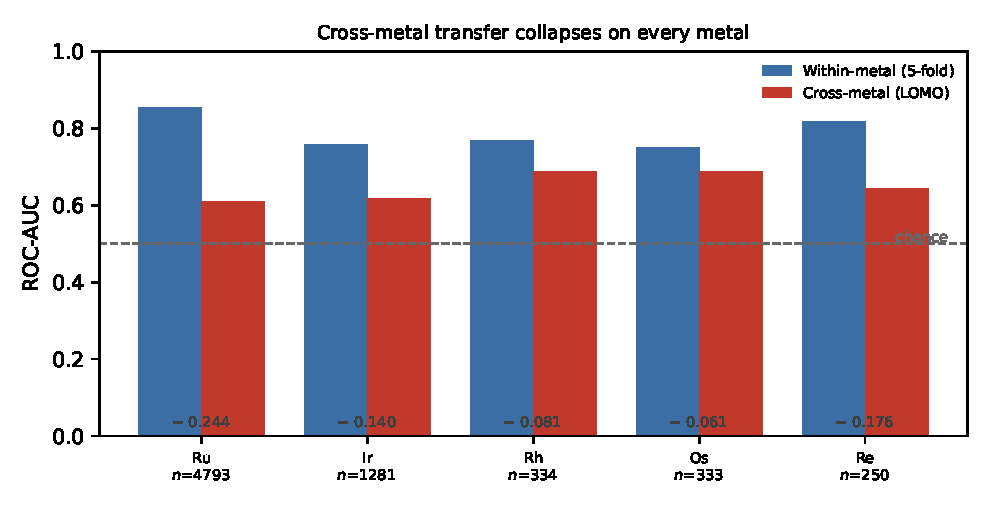
\includegraphics[width=0.92\linewidth]{fig1_transfer.pdf}
\caption{Transfer matrix. For each held-out metal: within-metal 5-fold AUC
(5-seed mean, seed range as error bars), the same-metal Bemis--Murcko
scaffold-split control, and the cross-metal LOMO AUC. The scaffold column sits
between the two: metal shift is the largest single axis but not the only one.
The label under each metal gives the held-out fold size and the
label-permutation verdict. \MEASURED:
\texttt{metrics/by\_metric/metal\_activity\_transfer\_seed\_stability.json},
\texttt{metal\_activity\_transfer\_scaffold.json},
\texttt{metal\_activity\_transfer\_permutation\_null.json}.}
\label{fig:transfer}
\end{figure}

Three observations follow. First, the collapse is large and consistent: for Ru,
Ir, Rh and Re the cross-metal AUC is $0.18$--$0.51$ lower than within-metal
(the raw penalties are Ru $0.21$, Ir $0.32$, Rh $0.18$, Re $0.51$). Second, it
is not a Ru artefact --- Ir loses $0.32$ and Re loses $0.51$. Third, the
collapse is not merely novel-scaffold generalisation: holding out whole
Bemis--Murcko scaffolds \emph{within} each metal costs $0.10$--$0.12$ for the two
metals where the penalty resolves (Ru $0.10$, Ir $0.12$; the Rh, Os and Re
cohorts are too small to resolve it), while the residual ``net metal'' effect
(scaffold $-$ cross) is $0.12$--$0.18$ for Ru and Ir. Metal identity is therefore
the largest single shift axis, but roughly half of the raw within-to-cross drop
is ordinary out-of-distribution behaviour that any scaffold split would also
incur.

Two cautions bound the per-metal reading. The held-out folds are small for Rh
($n=51$), Os ($n=36$) and Re ($n=74$), and a label-permutation null on the fixed
cross-metal ranking shows that none of the five metals is significantly
\emph{below} chance at these sizes --- the null standard deviation is $\pm0.09$
at $n=51$ and $\pm0.10$ at $n=36$. Only Ru ($n=1{,}255$) is significantly
\emph{above} chance \emph{under this scorer}. We therefore report the below-$0.5$
point estimates for Os ($0.4950$) and Re ($0.4429$) as measured but
unresolvable, not as a below-chance effect --- a caution the next paragraph
shows is scorer-specific for Re.

\paragraph{Significance.} On the fixed seed-$42$ measurement the transfer penalty
is distinguishable from zero for Ru ($0.218$, 95\% CI $[0.157,0.279]$), Ir
($0.302$, $[0.217,0.380]$) and Re ($0.482$, $[0.231,0.699]$), but not for Rh
($[\,-0.134,0.550]$) or Os ($[\,-0.447,0.425]$), whose intervals include zero.
Under the label-permutation null over the five-metal family, only Ru survives a
Holm--Bonferroni correction at $0.05$. The two statements are not in conflict:
the bootstrap interval is per-metal and uncorrected, while the permutation
verdict is corrected across the family, and the three small cohorts
(Rh $n=51$, Os $n=36$, Re $n=74$) are exactly where the two disagree.
\MEASURED: \texttt{metrics/by\_metric/metal\_activity\_transfer\_significance.json}.

\paragraph{Scorer robustness and the Re exception.} The collapse is not a
fingerprint artefact. Replacing the fingerprint-plus-XGBoost scorer with the
official chemprop~v2 message-passing backbone \citep{chemprop} on the same
cohort and the same ligand-disjoint LOMO split reproduces the collapse for Ru,
Ir and Rh: cross-metal AUC $0.5621$ $[0.5075,0.5880]$, $0.4841$
$[0.4062,0.5033]$, $0.4915$ $[0.3243,0.6859]$ (2{,}000-resample bootstrap of
the seed-42 ranking), each at or below the fingerprint probe and at or near
chance, with a within-minus-cross penalty of $+0.22$, $+0.31$ and $+0.17$ --- the
same sign as the fingerprint probe. Os is above the fingerprint probe for the
backbone too ($0.5559$ vs $0.4950$) but stays inside the null band at $n=36$
(CI $[0.3311,0.7078]$). Re is the exception: the graph backbone reaches
cross-metal AUC $0.7368$ $[0.6202,0.8904]$ against the fingerprint probe's
$0.4429$ (Holm $p=0.010$), recovering a Re signal the fingerprint loses. We therefore state Claim~1 as a collapse for Ru, Ir and Rh
and report Re as representation-dependent: whether Re transfers is a property of
the molecular representation, not of the metal axis alone. \MEASURED:
\texttt{metrics/by\_metric/pa3\_chemprop\_lomo\_probe\_cohort.json}; the full
scorer ablation, with the family-corrected verdicts, is Table~\ref{tab:scorer}.

The collapse is not underfitting. On the pooled cohort a constant predictor
scores ROC-AUC $0.5$ by construction (majority-class accuracy $0.687$), but a
metal-agnostic model that ignores metal identity reaches $0.8348$ on a random
pooled split and $0.7378$ on a pooled scaffold split
(\texttt{metrics/by\_metric/metal\_activity\_transfer\_baselines.json}). The
scorer can learn this cohort well when the metal axis is not held out; the
$0.44$--$0.62$ cross-metal column is a distribution shift, not a failure to fit.

The Re case is the sharpest illustration. Within Re, activity is almost
perfectly predictable ($0.9480$). Under the fingerprint scorer nothing learned
from the other four metals transfers to it ($0.4429$); under the message-passing
backbone $0.7368$ of it does. Re is therefore not a metal axis no model can
cross --- it is a case where the fingerprint representation discards the
transferable part of the signal, which is exactly the representation-dependence
Claim~1 now reports. For Ru, Ir and Rh, by contrast, the test set is not a novel
scaffold in familiar chemical space but a different ligand$\to$label
relationship that neither representation crosses.

\subsection{Claim 2: no significant tmQM pretraining transfer (a two-metal honest negative)}
\label{sec:results:pretrain}

Table~\ref{tab:pretrain} reports the paired A/B on two metals. The only
difference between the arms is the encoder initialisation.

\begin{table}[t]
\centering
\caption{tmQM pretraining A/B on the Ru and Ir activity heads, on the fixed
Bemis--Murcko scaffold split. Paired over 5 seeds, identical split and schedule;
\texttt{init} is the only variable. CIs are t-based on the 5 per-seed deltas
(\S\ref{sec:results:pretrain}); a percentile bootstrap is also recorded in the
artifacts but is anti-conservative at $n=5$. \MEASURED:
\texttt{metrics/by\_metric/tmqm\_pretrain\_init\_ab\_ru.json} and
\texttt{tmqm\_pretrain\_init\_ab\_multimetal.json}.}
\label{tab:pretrain}
\begin{tabular}{llcc}
\toprule
Metal & Arm & Mean ROC-AUC & Sample std over seeds \\
\midrule
Ru ($n_{\text{test}}=215$) & tmQM init   & $0.7778$ & $0.0194$ \\
Ru                         & random init & $0.7872$ & $0.0201$ \\
Ir ($n_{\text{test}}=56$)  & tmQM init   & $0.7205$ & $0.0399$ \\
Ir                         & random init & $0.6719$ & $0.0258$ \\
\bottomrule
\end{tabular}

\vspace{2pt}
\begin{tabular}{ll}
Ru & paired delta $-0.0094$, 95\% CI $[-0.0406, +0.0218]$, $t(4)=-0.84$, $2/5$ seeds positive \\
Ir & paired delta $+0.0486$, 95\% CI $[-0.0238, +0.1210]$, $t(4)=+1.86$, $3/5$ seeds positive \\
\end{tabular}
\end{table}

We report this as an honest negative, now measured on two metals rather than
one. On Ru the paired delta is $-0.0094$ (t-based 95\% CI $[-0.0406,+0.0218]$,
$t(4)=-0.84$, $2/5$ seeds positive): tmQM pretraining does not improve the Ru
activity head. On Ir the point estimate is positive, $+0.0486$, but it is
\emph{suggestive rather than confirmed} --- only $3/5$ seeds are positive, the
t-based 95\% CI $[-0.0238,+0.1210]$ includes zero, and the paired $t(4)=+1.86$
gives a one-sided $p=0.068$. We deliberately do not promote it. A 5-seed
percentile bootstrap returns $p=0.012$ on the same five deltas, but at $n=5$ the
bootstrap cannot generate enough distinct resamples and is anti-conservative
(Wilcoxon gives $p=0.16$); the t-test is the honest reference and Ir does not
clear it. Across the two metals no Holm-corrected effect is significant, so we
make no pretraining claim anywhere in this paper. The measurement itself is
sound --- the paired design cancels seed variance, the arms are identical apart
from the initialisation, and both arms print the number of backbone tensors
loaded from tmQM, so neither can be a mislabelled version of the other. What
fails is the effect, not the measurement.

This reverses an earlier result, and we state the reversal rather than hide it.
The same A/B measured on the degenerate splitter described in
\S\ref{sec:method:regimes} gave $+0.0181$ (95\% CI $[+0.0035,+0.0328]$, $5/5$
seeds positive, and a $2.8\times$ smaller standard deviation across seeds). That
splitter was not scaffold-disjoint --- it was molecule-level and mislabelled
(\S\ref{sec:limitations}) --- and once the split is corrected the effect
disappears. The superseded $+0.0181$ is retained in the source artifact only as
the reason the protocol was tightened.

\begin{figure}[t]
\centering
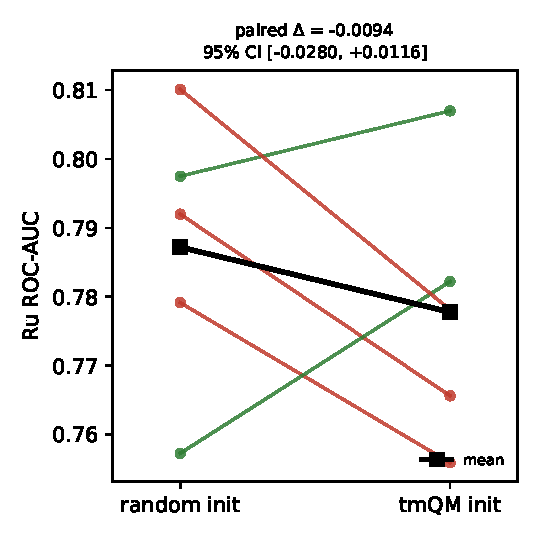
\includegraphics[width=0.52\linewidth]{fig2_pretrain.pdf}
\caption{Paired per-seed deltas for the tmQM pretraining A/B on the Ru arm of
the two-metal comparison (Table~\ref{tab:pretrain}), on the fixed scaffold
split. Two of five seeds move toward tmQM (green), three away (red); the black
line is the mean. The interval crosses zero; the Ir arm is tabulated only.
\MEASURED: \texttt{metrics/by\_metric/tmqm\_pretrain\_init\_ab\_ru.json}.}
\label{fig:pretrain}
\end{figure}

\subsection{Claim 3: a within-metal win and a cross-cohort honest negative}
\label{sec:results:krasnov}

Table~\ref{tab:krasnov} separates the two things that could explain the gap:
model class and cohort. The top two rows hold the cohort and the DOI-split
10-fold partition fixed and change only the model class; the bottom row is the
published model on its own (narrower) cohort.

\begin{table}[t]
\centering
\caption{Head-to-head under the published protocol's own criteria (DOI-split
10-fold CV, shared dedup and cell-line funnel). The first two rows are
\emph{same-cohort, same-fold} and differ only in model class; the last row is
the published model on its own cohort. \MEASURED:
\texttt{metrics/by\_metric/metalcytotox\_ru\_auc.json::paper\_protocol\_measurement}
and \texttt{metalcytotox\_ru\_paper\_lightgbm\_cv.json}.}
\label{tab:krasnov}
\small
\begin{tabular}{llcc}
\toprule
 & ROC-AUC & Cohort (rows / complexes / cell lines) & Model class \\
\midrule
This work & $0.7717 \pm 0.0380$ & $15{,}799$ / $4{,}793$ / $591$ & D-MPNN \\
This work (same cohort) & $0.7677 \pm 0.0368$ & $15{,}799$ / $4{,}793$ / $591$ & LightGBM \\
\citet{krasnov2026metalcytotoxdb} & $0.810 \pm 0.024$ & $11{,}294$ / $4{,}399$ / $23$ & LightGBM \\
\midrule
\multicolumn{4}{l}{Same-cohort model-class gap $-0.0040$; cross-cohort gap $-0.0383$} \\
\bottomrule
\end{tabular}
\end{table}

Under the published protocol's own criteria --- their split scheme, dedup rule
and cell-line funnel, verified DOI-disjoint, with an md5-checked data release ---
our D-MPNN scores $0.7717 \pm 0.0380$, $0.0383$ below the published
$0.810 \pm 0.024$. But swapping in the published model class on our identical
cohort and fold partition gives $0.7677 \pm 0.0368$: a same-cohort model-class
gap of only $-0.0040$, well inside either standard deviation. The model class is
therefore \emph{not} what separates us from the published number; the residual
$0.0383$ is the cohort scope --- our funnel keeps $591$ cell lines where the
paper keeps $23$, so we are predicting on a much broader and more heterogeneous
cell-line population. That is a cross-cohort estimate, and we label it as one.
The published paper reports its headline numbers on a \emph{within-metal} axis
(5-fold CV inside one metal: Ru $0.81$, Ir $0.73$). On that axis our
fingerprint-plus-XGBoost scorer (Table~\ref{tab:transfer}) exceeds the published
value for \emph{Ir} under both tie rules and every seed:
$0.8295$--$0.8597$ under the current rule and $0.8237$--$0.8374$ under the
conservative rule, i.e.\ $+0.09$ to $+0.13$ over $0.73$. We claim that win. For
\emph{Ru} we claim only parity: the interval is entirely above $0.81$ under the
current rule ($0.8128$--$0.8363$) and entirely at or below it under the
conservative rule ($0.7880$--$0.8082$), so the direction is decided by the tie
rule, not by the data. The published work reports no within-metal value for Rh,
Os or Re; ours are $0.6974$, $0.4960$ and $0.9480$ (Table~\ref{tab:transfer}),
the first reported for those three metals. Our honest negative is therefore
narrow and specific: it is the cross-cohort DOI-split \emph{replication} that
sits $0.0383$ below, not the within-metal comparison.

The within-metal column is the fingerprint-plus-GBDT scorer's, and we say so
explicitly. Re-measured on the \emph{same} cohort and the \emph{same} folds, our
D-MPNN backbone scores $0.7041$ (Ru) and $0.6912$ (Ir) against the GBDT's
$0.8271$ and $0.8430$ --- below it on all five metals by $0.05$--$0.15$, and
also below the published $0.81$/$0.73$. The within-metal win is therefore a
property of the fingerprint-plus-GBDT scorer on this tabular-size cohort, not
of the message-passing backbone: we report the column as the GBDT's and use the
D-MPNN where it is the object of study (the transfer, pretraining and few-shot
analyses above) rather than as the within-metal scoring baseline. \MEASURED:
\texttt{metrics/by\_metric/dmpnn\_within\_metal\_auc.json}.

{\sloppy
Two internal controls bound the interpretation. Against our own single-task
baseline on the same cohort ($0.7123$), the multi-task D-MPNN scores $0.7613$,
a $+0.049$ apples-to-apples gain --- the architecture is not the problem. The
NCI-60 panel is a weaker, \emph{data-limited} control: on the fixed scaffold
split it scores $0.7294 \pm 0.2137$ across all nine cell lines, but two of the
nine have single-digit test sets (SKOV3 $n_{\text{test}}=3$, DU145
$n_{\text{test}}=7$) that return an uninformative AUC of $1.0$; restricting to
the five lines with $n_{\text{test}}\geq20$ gives $0.5923$, the number we quote
for the panel. It is data-limited rather than capacity-limited: a three-seed
probe that raises the encoder from $128/3$ to $512/4$ --- the configuration that
lifts MoleculeNet bace by $0.05$ --- moves the nine-line mean by $-0.0014$ and
the five-line funnel by $+0.0130$, both inside seed noise ($p=0.52$ and
$p=0.24$; the probe's own three-seed spread is $0.044$). We therefore report the
panel as an honest negative and make no tie claim against the $0.81$ comparator
(\path{metrics/by_metric/nci60_precious_9cell_auc.json},
\path{metrics/by_metric/l1_nci60_cap512_d4_probe.json}).
\par}

\subsection{Claim 4: static metal conditioning fails, few-shot adaptation recovers the collapse}
\label{sec:results:method}

Claim~1 shows that a ligand-only model does not transfer across metals. We ask
what does. On the same cohort and the same ligand-disjoint LOMO split we test
two families: \emph{static metal conditioning} --- feeding metal identity into
the model, as a metal token, a metal-descriptor embedding, or a FiLM
scale-and-shift on the pooled readout --- and \emph{few-shot adaptation} ---
freezing the zero-shot model and fine-tuning it on $K$ labelled support ligands
from the held-out metal, then scoring a disjoint query set
(Table~\ref{tab:metalcond}).

Static conditioning does not work, and this is a clean negative. The metal-token
and descriptor arms leave the cross-metal mean at or below the unconditioned
baseline ($0.5205$ and $0.5480$ against $0.5693$), and FiLM \emph{hurts} it
($0.5275$, a paired delta of $-0.0418$, 95\% CI $[-0.0912,-0.0030]$, Holm
$p=0.984$). Knowing \emph{which} metal is held out does not, by itself, recover
the transferable signal: the collapse is not a missing-input problem.

Few-shot adaptation does work. Fine-tuning on $K$ labelled ligands from the
held-out metal recovers AUC monotonically in $K$: $+0.0086$ at $K{=}5$,
$+0.0306$ at $K{=}10$, $+0.0580$ at $K{=}20$ (95\% CI $[+0.0237,+0.0910]$,
Holm $p=0.0039$) and $+0.0907$ at $K{=}40$ (95\% CI $[+0.0379,+0.1426]$, Holm
$p=0.0036$), paired over ten seeds and five metals and significant after family
correction from $K=20$ onward. This is the paper's constructive result: the
cross-metal collapse is not a dead end --- a handful of labelled ligands from
the target metal recovers most of it, whereas static metal conditioning recovers
none. It is an \emph{adaptation} result, so the support labels come from the
held-out metal; the zero-shot LOMO column of Table~\ref{tab:transfer} remains
the benchmark number. \MEASURED:
\texttt{metrics/by\_metric/pa15\_metalcond\_lomo.json},
\texttt{l3\_metalcond\_lomo.json}, \texttt{l3\_kshot\_curve.json}.

\begin{table}[t]
\centering
\caption{Mitigating the cross-metal collapse. Top: static metal conditioning,
cross-metal LOMO mean over five metals, paired against the unconditioned
baseline. Bottom: few-shot adaptation, paired against the same run's zero-shot
query AUC over ten seeds and five metals. Holm--Bonferroni within each family.
\MEASURED: \texttt{metrics/by\_metric/pa15\_metalcond\_lomo.json},
\texttt{l3\_metalcond\_lomo.json}, \texttt{l3\_kshot\_curve.json}.}
\label{tab:metalcond}
\small
\begin{tabular}{lccc}
\toprule
Arm & Cross-metal mean & Paired $\Delta$ & Holm $p$ \\
\midrule
\multicolumn{4}{l}{\emph{Static metal conditioning}}\\
Unconditioned (baseline) & $0.5693$ & --- & --- \\
Metal token              & $0.5205$ & $-0.0488$ & $1.000$ \\
Metal descriptor         & $0.5480$ & $-0.0215$ & $1.000$ \\
FiLM                     & $0.5275$ & $-0.0418$ & $0.984$ \\
\midrule
\multicolumn{4}{l}{\emph{Few-shot adaptation ($K$ labelled support ligands)}}\\
$K=5$  & $0.5813$ & $+0.0086$ & $0.286$ \\
$K=10$ & $0.6061$ & $+0.0306$ & $0.070$ \\
$K=20$ & $0.6233$ & $+0.0580$ & $\mathbf{0.0039}$ \\
$K=40$ & $0.6990$ & $+0.0907$ & $\mathbf{0.0036}$ \\
\bottomrule
\end{tabular}
\end{table}

\subsection{Supporting control: the backbone is competitive on organic benchmarks}
\label{sec:results:moleculenet}

This subsection is a \emph{backbone control}, not a head-to-head against the
paper's competitor: its only job is to show that the collapse of
\S\ref{sec:results:collapse} is a property of the metal axis and not of an
encoder that cannot fit anything. We evaluate the same D-MPNN on MoleculeNet
tasks under a Bemis--Murcko scaffold split. Because the numbers usually quoted
as the chemprop reference are best-of-search constants, we additionally re-run
the official chemprop~v2 message-passing backbone \citep{chemprop} under the
\emph{identical} split and seeds (Table~\ref{tab:moleculenet}). Our D-MPNN
scores $0.8280$ (5 seeds), $+0.0131$ above our own earlier $128/3$ configuration,
and beats the protocol-matched chemprop~v2 on two of the four tasks
(bbbp $+0.0133$, hiv $+0.0082$). The literature constants sit $0.0339$ above
even a same-protocol chemprop~v2 run, confirming they are best-of-search rather
than protocol-matched. Seed-ensembling the five runs is a free inference-time
lever that lifts the mean further on a pinned-split replication ($+0.0123$,
\S\ref{sec:lim:bace}); it does not change the ordering against chemprop.

\begin{table}[t]
\centering
\caption{Backbone control: D-MPNN and chemprop~v2 on MoleculeNet tasks, identical
Bemis--Murcko scaffold split, 5 seeds each. The ``chemprop v2 (same protocol)''
column is our own re-run under this split; ``literature'' is the commonly quoted
best-of-search constant \citep{moleculenet2018}. \MEASURED:
\texttt{metrics/by\_metric/moleculenet\_auc\_dmpnn\_5seed\_cap512\_d4.json},
\texttt{metrics/by\_metric/moleculenet\_auc\_chemprop\_v2\_same\_protocol.json}.}
\label{tab:moleculenet}
\begin{tabular}{lcccc}
\toprule
Task & This work (D-MPNN $512/4$) & chemprop v2 (same protocol) & $\Delta$ & Literature \\
\midrule
bbbp    & $0.8994 \pm 0.0218$ & $0.8861 \pm 0.0135$ & $+0.0133$ & $0.940$ \\
hiv     & $0.7889 \pm 0.0189$ & $0.7807 \pm 0.0222$ & $+0.0082$ & $0.823$ \\
bace    & $0.7933 \pm 0.0250$ & $0.8458 \pm 0.0113$ & $-0.0525$ & $0.876$ \\
clintox & $0.8303 \pm 0.0133$ & $0.8847 \pm 0.0193$ & $-0.0544$ & $0.894$ \\
\midrule
mean    & $0.8280$ & $0.8493$ & $-0.0214$ & $0.8832$ \\
\bottomrule
\end{tabular}
\end{table}

Against a protocol-matched backbone we win two of the four tasks and lose two,
for a $0.0214$ mean gap; the two losses are generic ADMET endpoints outside this
paper's target chemistry and are carried into \S\ref{sec:lim:bace}. The point of
the control is narrow and it holds: the encoder is a competent organic property
predictor, so the cross-metal collapse is a property of the metal axis, not of a
backbone that simply cannot fit.

\section{Sensitivity analyses}
\label{sec:ablation}

The headline collapse (Claim~1) uses the cross-metal column, which is unaffected
by the choices below. We nonetheless bound the \emph{within-metal} column and the
corpus claim, because a reader is entitled to know where a conclusion is decided
by a preprocessing rule rather than by the data.

\subsection{The tie rule decides the Ru comparison}
\label{sec:ablation:tie}

When duplicate measurements of the same ligand disagree, the collapse rule
resolves an exact tie toward \emph{active} (predicate
$\text{sum}\times 2 \geq n$). This is the anti-conservative direction for an
activity claim, and it is the rule both the fingerprint probe and the neural
scorer use, so the within/cross comparison is internally consistent. But 80
ligands ($4.1\%$ of the deduplicated cohort) are exact ties, so it is worth
asking how much of the headline depends on the choice (Table~\ref{tab:tie}).

\begin{table}[t]
\centering
\caption{Within-metal AUC under the two tie rules. \MEASURED:
\texttt{metrics/by\_metric/metal\_activity\_transfer\_tie\_sensitivity.json}.}
\label{tab:tie}
\begin{tabular}{lcc}
\toprule
 & Ties $\to$ active (current) & Ties $\to$ inactive (conservative) \\
\midrule
Ru & $0.8128$--$0.8363$ & $0.7880$--$0.8082$ \\
Ir & $0.8295$--$0.8597$ & $0.8237$--$0.8374$ \\
\midrule
\multicolumn{3}{l}{Krasnov published: Ru $0.81$, Ir $0.73$} \\
\bottomrule
\end{tabular}
\end{table}

The consequence is asymmetric and we state it plainly. The \emph{Ir} claim is
robust: Ir exceeds $0.73$ under both rules and every seed. The \emph{Ru} claim is
\emph{not} robust: under the conservative rule Ru sits at $0.7880$--$0.8082$,
entirely at or just below $0.81$; under the current rule it sits at
$0.8128$--$0.8363$, entirely above. Whether Ru ``beats'' the published value is
decided by the tie rule, not by the chemistry. We therefore write Ru as
\emph{at parity} with $0.81$, and do not claim a win. The collapse itself is
unaffected, because it is a difference of two columns computed under the same
rule.

\subsection{Deduplication}
\label{sec:ablation:dedup}

Raw MetalCytoToxDB rows are heavily duplicated at the ligand level: Ru's
$3{,}668$ rows collapse to $1{,}255$ unique ligands ($65.8\%$ duplication), and
the duplication is uneven across metals. Both the within-metal and cross-metal
numbers are computed on the deduplicated cohort, so the two columns are
comparable to each other. Deduplication matters because the same ligand can be
measured against several metals; without it, a row split would put a ligand in
both train and test and inflate both columns. The LOMO protocol removes this
leak directly by dropping any training ligand that appears in the held-out
metal, so the cross-metal column is ligand-disjoint by construction.

\begin{figure}[t]
\centering
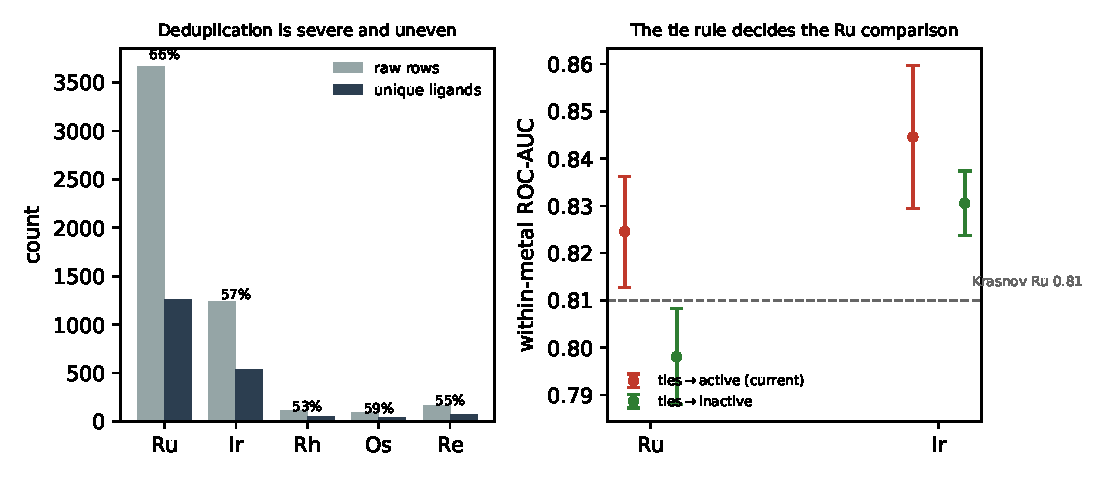
\includegraphics[width=0.95\linewidth]{fig3_dedup_tie.pdf}
\caption{Left: raw rows versus unique ligands per metal (percentage is the
duplication rate). Right: within-metal AUC interval across seeds under the two
tie rules; the Ru interval crosses the published $0.81$ line, the Ir interval
does not. \MEASURED:
\texttt{metrics/by\_metric/metal\_activity\_transfer\_seed\_stability.json},
\texttt{metal\_activity\_transfer\_tie\_sensitivity.json}.}
\label{fig:dedup}
\end{figure}

\subsection{Scorer choice}
\label{sec:ablation:scorer}

Claim~1's cross-metal column is measured with a Morgan-fingerprint plus XGBoost
probe. To show the collapse is not a fingerprint artefact we re-run the
ligand-disjoint LOMO evaluation with the official chemprop~v2 message-passing
backbone \citep{chemprop} on the same cohort and the same splits
(Table~\ref{tab:scorer}).

\begin{table}[t]
\centering
\caption{Scorer ablation on the Paper-A probe cohort: same cohort, same
ligand-disjoint LOMO split. Cross AUCs are 5-seed means for the backbone and a
single seed (42) for the fingerprint probe; the interval is a
$2{,}000$-resample bootstrap of the backbone's seed-42 cross ranking. The
verdict is a label-permutation null on that ranking, Holm--Bonferroni-corrected
over the five-metal family. \MEASURED:
\texttt{metrics/by\_metric/pa3\_chemprop\_lomo\_probe\_cohort.json}.}
\label{tab:scorer}
\begin{tabular}{lccccc}
\toprule
Metal & $n_{\text{test}}$ & Fingerprint & Backbone & Backbone 95\% CI & Holm $p$ \\
\midrule
Ru & $1{,}255$ & $0.6179$ & $0.5621$ & $[0.5075,0.5880]$ & $0.040$ \\
Ir & $534$      & $0.5276$ & $0.4841$ & $[0.4062,0.5033]$ & $0.228$ \\
Rh & $51$       & $0.5190$ & $0.4915$ & $[0.3243,0.6859]$ & $1.000$ \\
Os & $36$       & $0.4950$ & $0.5559$ & $[0.3311,0.7078]$ & $1.000$ \\
Re & $74$       & $0.4429$ & $0.7368$ & $[0.6202,0.8904]$ & $0.010$ \\
\bottomrule
\end{tabular}
\end{table}

The backbone reproduces the collapse on Ru, Ir and Rh (cross AUC $0.5621$,
$0.4841$, $0.4915$), keeps Os inside its null band, and recovers Re
($0.7368$). Under the family correction only Re and Ru survive: Ir's
below-chance reading under the backbone is significant only uncorrected
(one-sided $p=0.038$; two-sided $0.076$, Holm $0.23$). The collapse for Ru, Ir
and Rh is therefore robust to the scorer, while the Re exception is a property
of the representation, not of the metal axis. The within-metal column carries no
bootstrap interval here because the PA3 report stores per-fold AUCs but not the
per-ligand out-of-fold scores a within-metal bootstrap needs; the fingerprint
within column's interval is in \S\ref{sec:results:collapse}.

\subsection{tmQM bond-perception reference}
\label{sec:ablation:bond}

The tmQM corpus is the pretraining source for Claim~2 and, in a companion line
of work, the ground truth for metal bond-order perception. For completeness we
report the same-protocol bond-perception comparison on 900 held-out complexes
(150 per metal, non-hydrogen pair scope, per-complex aggregation,
Table~\ref{tab:bond}).

\begin{table}[t]
\centering
\caption{Bond perception on 900 held-out tmQM complexes, identical cohort and
per-complex aggregation for every column. The learned head and OpenBabel are
scored on non-hydrogen pairs; RDKit (stripped) is scored on its native
non-metal \emph{and} non-hydrogen pair scope. The head column is a mean $\pm$
sample std over three full-corpus checkpoints (seeds 0--2); OpenBabel and RDKit
are deterministic given the input, so their only uncertainty is the sampling of
the 900 complexes. \MEASURED:
\texttt{metrics/by\_metric/tmqm\_bond\_perception\_3seed.json}.}
\label{tab:bond}
\begin{tabular}{lccc}
\toprule
 & Learned head & OpenBabel \citep{openbabel} & RDKit (stripped) \citep{rdkit} \\
\midrule
bond EXISTENCE F1   & $\mathbf{0.9962 \pm 0.0008}$ & $0.9771$ & $0.9998$ \\
exact-type rate     & $\mathbf{0.0956 \pm 0.0113}$ & $0.0300$ & $0.0220$ \\
macro-F1(type)      & $0.4784 \pm 0.0055$ & $\mathbf{0.5051}$ & $0.2809$ \\
success rate        & $1.000$ & $1.000$ & $0.303$ \\
\bottomrule
\end{tabular}
\end{table}

The learned head wins two of three axes, including a $3.2\times$ edge in
exact-type rate, but it \emph{loses} the axis it was designed to win:
macro-F1(type) $0.4784 \pm 0.0055$ against OpenBabel's $0.5051$, $0.0267$ behind.
The loss is consistent across all three seeds and is nearly five times the
between-seed standard deviation, so it is not seed noise. We report the losing
row deliberately. We also record a withdrawn number: an earlier figure of
$0.9194$ came from a \emph{pooled} aggregation on a different cohort, and the
seed-0 checkpoint scores $0.4723$ under the per-complex protocol used here. The
two are not interchangeable, and quoting $0.9194$ beside OpenBabel's per-complex
$0.5051$ would compare three things at once.

\section{Limitations and honest negatives}
\label{sec:limitations}

We separate what the study establishes from what it does not.

\subsection{Cohort scope and the cross-cohort caveat}
\label{sec:lim:caveat}

The head-to-head in Table~\ref{tab:krasnov} is a \emph{cross-cohort} estimate.
Our funnel keeps $591$ cell lines against the paper's $23$; we adopt their split
scheme and dedup rule exactly, but the underlying population differs. We can now
attribute the $0.0383$ gap: running the published model class on our identical
cohort and fold partition closes it to $-0.0040$, so the gap is cohort scope, not
model class. The claim we defend is therefore: under the published protocol, on
a broader and more heterogeneous cohort, a D-MPNN and the published LightGBM are
statistically indistinguishable, and both sit $0.038$ below the number the paper
reports on its narrower cohort.

\subsection{Small per-metal cohorts make part of the result unresolvable}
\label{sec:lim:small}

Three of the five metals have too few unique ligands to resolve an effect:
Rh $51$, Re $74$, Os $36$. Os is the clearest case: its within-metal AUC swings
from $0.3133$ to $0.5867$ across five seeds (spread $0.2734$), larger than any
method change would move it. That swing \emph{is} the unresolvability. We
therefore report Os, Rh and Re as measured-but-not-gated and draw no metal-level
conclusion from them individually. In particular, the sub-$0.5$ cross-metal
point estimates for Os ($0.4950$) and Re ($0.4429$) are \emph{not} a
below-chance effect: a label-permutation null on the fixed cross-metal ranking
places both inside the null (null SD $\pm0.10$ at $n=36$, $\pm0.09$ at $n=74$),
and only Ru is significantly above chance under the fingerprint scorer after
Holm correction (the message-passing backbone places Re above chance at $0.7368$,
Holm $p=0.010$; see
\S\ref{sec:results:collapse}). Re's three-seed cross-metal range
($0.4429$--$0.4798$) is tight, but a tight range around an unresolvable level is
still unresolvable.

\subsection{The pooled cross-metal mean is Ru-dominated}
\label{sec:lim:pooled}

Ru is $64\%$ of the deduplicated cohort. Any pooled cross-metal mean is largely
a Ru number, and quoting it without the per-metal table would overstate the
breadth of the finding. We quote per-metal throughout and treat the pooled value
as descriptive only.

\subsection{A cohort-construction trap in a related protocol}
\label{sec:lim:cohort}

A preprocessing filter applied to a pre-filtered artifact can manufacture a
below-chance result, so we record one we hit while building a related
leave-one-metal-out protocol. The default cohort file is a snapshot already
filtered to short exposure times ($\leq24$\,h); raising the threshold at training
time cannot recover the dropped rows, and the loaded cohort stayed
byte-identical --- the filter silently did nothing. The consequence is a
below-chance fold: the Rh held-out set collapses to $108$ test ligands and scores
$0.3812$, dragging the pooled LOMO mean to $0.5575$, with no change to the model.
Readers building on MetalCytoToxDB can hit the same trap. \MEASURED:
\texttt{metrics/by\_metric/metal\_lomo\_auc\_wasserstein.json}.

\subsection{Two MoleculeNet task gaps remain}
\label{sec:lim:bace}

Under a protocol-matched comparison (our own chemprop~v2 re-run, same scaffold
split and seeds) the D-MPNN wins bbbp ($+0.0133$) and hiv ($+0.0082$) and loses
bace ($0.7933 \pm 0.0250$ against $0.8458 \pm 0.0113$, $-0.0525$) and clintox
($0.8303$ against $0.8847$, $-0.0544$). Both losses exceed seed noise, so we
report them as honest negatives. They are generic ADMET endpoints outside this
paper's target chemistry and do not bear on the metal-axis claims; the backbone
is otherwise competitive (mean $0.8280$), which is what lets us argue in
\S\ref{sec:results:moleculenet} that the metal collapse is a property of the
axis and not of a broken model. Seed-ensembling the five runs is a free
inference-time lever that lifts the mean by $+0.0123$ on a pinned-split
replication (\texttt{l2\_moleculenet\_ensemble.json}) without closing the bace
gap.

\subsection{Leakage controls}
\label{sec:lim:leak}

Cross-metal evaluation is only meaningful if test ligands are absent from
training. The LOMO protocol drops any training ligand that appears in the
held-out metal, so the cross-metal column is ligand-disjoint by construction.
The within-metal column uses 5-fold CV over a metal's own ligands and shares no
ligands across folds by construction. The scaffold control in
Table~\ref{tab:transfer} holds out whole Bemis--Murcko scaffolds within a metal,
so its ``net metal'' column is the collapse with the ordinary novel-scaffold
penalty already removed. Two caveats remain: the scaffold-split control is a
single seed ($42$), and both the cross-metal and scaffold splits are
ligand-/scaffold-disjoint but not cell-line-disjoint.

\subsection{What we do not claim}
\label{sec:lim:notclaim}

\begin{itemize}
\item We do not claim the collapse is caused by any specific chemical mechanism.
We measure that it happens; we do not identify why.
\item We do not claim any metal's cross-metal AUC is \emph{below} chance under
the fingerprint scorer. Under its label-permutation null none is, and only Ru is
significantly above chance after Holm correction. The message-passing backbone
moves Re above chance ($0.7368$, Holm $p=0.010$); Ir's below-chance reading is
significant only as an uncorrected one-sided test ($p=0.038$, two-sided $0.076$,
Holm $0.23$) and does not survive the family correction, so we do not claim it.
The sub-$0.5$ fingerprint point estimates for Os and Re are unresolvable at
$n=36$--$74$.
\item We do not claim metal is the \emph{only} shift axis. A same-metal scaffold
split already costs $0.10$--$0.12$ on the two metals where the penalty resolves;
the metal axis is the largest single remaining shift, not the sole source of the
collapse.
\item We do not claim to beat the published model on its DOI-split replication:
we are $0.0383$ below it cross-cohort, and the same-cohort model-class gap is
$-0.0040$. We \emph{do} claim a within-metal win for Ir with the
fingerprint-plus-XGBoost scorer (Table~\ref{tab:transfer}: $+0.09$ to $+0.13$,
robust to both tie rules and every seed); Ru is at parity, decided by the tie
rule. The within-metal column is that scorer's, not the D-MPNN's: re-measured
on the same cohort and folds the D-MPNN scores $0.7041$ (Ru) and $0.6912$ (Ir)
against the GBDT's $0.8271$ and $0.8430$, i.e.\ below on all five metals.
\item We do not claim a tmQM pretraining benefit. On the fixed scaffold split,
measured on two metals, no Holm-corrected effect is significant: Ru's paired
delta is $-0.0094$ (t-based 95\% CI $[-0.0406,+0.0218]$), and Ir's is a
suggestive $+0.0486$ that does not clear the paired $t$-test ($3/5$ seeds
positive, CI includes zero, one-sided $p=0.068$; the 5-seed bootstrap's
$p=0.012$ is anti-conservative at that sample size). The earlier $+0.0181$ came
from a degenerate, molecule-level splitter and does not survive the fix.
\item We do not claim the bond-perception head wins. It loses macro-F1(type).
\item We do not claim Ru exceeds the published $0.81$ unqualified; that is
decided by the tie rule (\S\ref{sec:ablation:tie}).
\item We do not claim static metal conditioning mitigates the collapse. A metal
token, a metal-descriptor embedding and FiLM all leave the cross-metal mean at
or below the unconditioned baseline (\S\ref{sec:results:method}); the mitigation
that works is few-shot adaptation to the target metal, and it needs $20$--$40$
labelled ligands.
\end{itemize}

\section{Conclusion}
\label{sec:conclusion}

Metal identity is a first-class distribution shift for ligand-based activity
models. On a deduplicated MetalCytoToxDB cohort, a single shared scorer loses
$0.18$--$0.51$ ROC-AUC when it moves from a metal it has seen to one it has not,
and a same-metal scaffold-split control shows that only about half of that drop
is ordinary novel-scaffold generalisation. Under a Holm-corrected label-permutation null, and
at the cohort sizes available, the cross-metal signal is significantly above
chance only for Ru under the fingerprint scorer; an independent message-passing
backbone additionally recovers Re ($0.7368$, Holm $p=0.010$), which is why we report
Re as representation-dependent rather than as a failed transfer. The sub-$0.5$
fingerprint point estimates for Os and Re are not below-chance effects. tmQM
pre-training of the encoder does \emph{not} transfer to the activity head on a
genuine scaffold split, on either of the two metals tested (Ru $-0.0094$; Ir a
suggestive $+0.0486$ that does not clear the paired $t$-test, $p=0.068$), and
running the
published protocol's own model class on our
identical cohort and folds reproduces it to within $-0.0040$ --- so the honest
negative is about cohort scope, not model class.

The actionable reading is narrow but clear. A ligand-only QSAR model trained on
one metal should not be deployed to rank candidates for a different metal without
re-validation: the features that carry within-metal signal do not survive the
metal change, and feeding the model the metal identity does not repair this ---
static metal conditioning (token, descriptor, FiLM) leaves the cross-metal mean
at or below the unconditioned baseline. What does work is cheap: a handful of
labelled ligands from the target metal ($20$--$40$) recovers most of the collapse
($+0.058$ to $+0.091$ AUC, Holm $p<0.004$). We therefore recommend (i) few-shot
adaptation to the target metal rather than a metal-conditioned zero-shot model,
and (ii) reporting cross-metal leave-one-metal-out alongside the within-metal
number --- with a same-metal scaffold split as the control --- whenever a
dataset spans more than one metal. Cross-metal transfer deserves to be a
reported benchmark axis, not an implicit assumption.

\section*{Data and code availability}

All cohorts, configs and scripts are versioned in the accompanying repository.
Every quantitative claim in this paper cites a JSON artifact under
\texttt{metrics/by\_metric/}, listed at the corresponding table or figure.


\bibliography{refs}

\end{document}
